\documentclass[10pt,a4paper]{report}
\usepackage[utf8]{inputenc}
\usepackage[russian]{babel}
\usepackage{amsmath}
\usepackage{amsfonts}
\usepackage{amssymb}
\usepackage{graphicx}
\author{Скрипаль Борис}
\title{Лабораторная работа №1.\\
	Программа для шифрования и подписи GPG, пакет Gpg4win}
\begin{document}
\maketitle
\renewcommand{\thesection}{\arabic{section}}
\tableofcontents
\pagebreak

\setcounter{totalnumber}{10}
\setcounter{topnumber}{10}
\setcounter{bottomnumber}{10}
\renewcommand{\topfraction}{1}
\renewcommand{\textfraction}{0}

\section{Цель работы}
Научиться создавать сертификаты, шифровать файлы и ставить ЭЦП.
\section{Описание лабораторной работы}
Электронная цифровая подпись (ЭЦП) — реквизит электронного документа, полученный в результате криптографического преобразования информации с использованием закрытого ключа подписи и позволяющий проверить отсутствие искажения информации в электронном документе с момента формирования подписи (целостность), принадлежность подписи владельцу сертификата ключа подписи (авторство), а в случае успешной проверки подтвердить факт подписания электронного документа (неотказуемость).

В данной лабораторной работе для генерации ЭЦП будет использоваться набор утилит, реализующих стандарт OpenPGP (Kleopatra, GPG4win и др.).
\section{Ход работы}
\subsection{Создание сертификата openPGP}
Для создания новой ключевой пары OpenPGP необходимо открыть графическую оболочку \textit{"Kleopatra"} и выполнить команду \textit{"File \begin{math}\to\end{math} New Certificate"}. После чего откроется помощник (рисунок \ref{ris:step11}).

\begin{figure}[h]
	\center{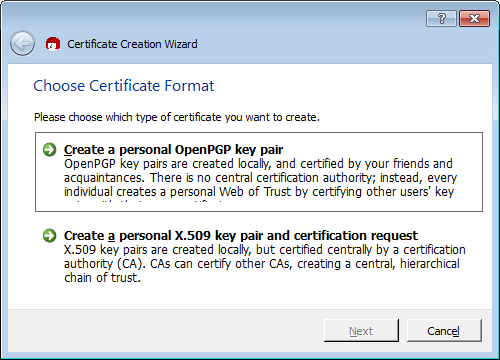
\includegraphics[width=1\linewidth]{res/step11}}
	\caption{Окно выбора типа сертификата безопасности.}
	\label{ris:step11}
\end{figure}

В данном случае необходимо выбрать первый пункт (\textit{Create a personal OpenPGP key pair}), после чего откроется окно ввода информации о пользователе (рисунок \ref{ris:step12}).

\begin{figure}[h]
	\center{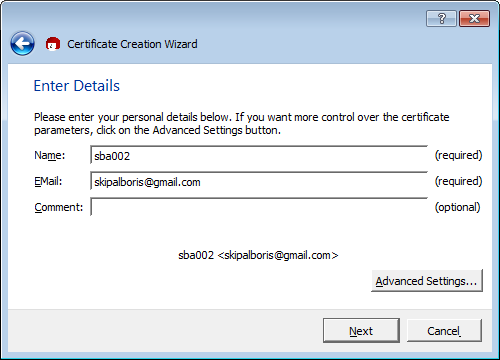
\includegraphics[width=1\linewidth]{res/step12}}
	\caption{Окно ввода информации о пользователе.}
	\label{ris:step12}
\end{figure}

После ввода личных данных необходимо ввести фразу-пароль (рисунок \ref{ris:step13}).

\begin{figure}[h]
	\center{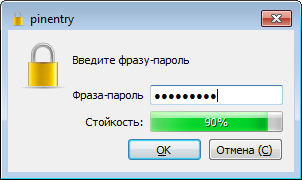
\includegraphics[width=0.6\linewidth]{res/step13}}
	\caption{Окно ввода фразы - пароля.}
	\label{ris:step13}

\end{figure}

После выполнения данных шагов, помощник выведет сообщение об успешном создании ключевой пары (рисунок \ref{ris:step14}).

\begin{figure}[h]
	\center{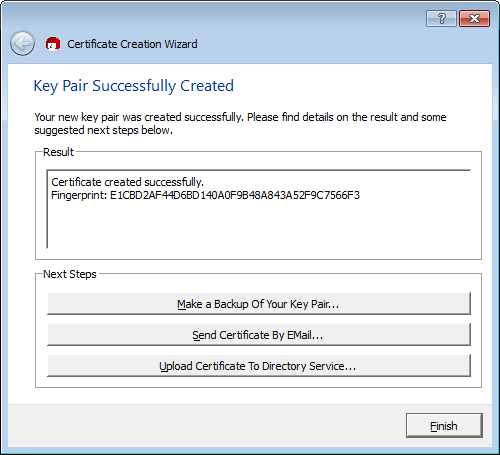
\includegraphics[width=1\linewidth]{res/step14}}
	\caption{Окно оповещения об успешном создании ключевой пары.}
	\label{ris:step14}
\end{figure}

Так же новая ключевая пара появится в рабочем пространстве (рисунок \ref{ris:step15}).

\begin{figure}[h]
	\center{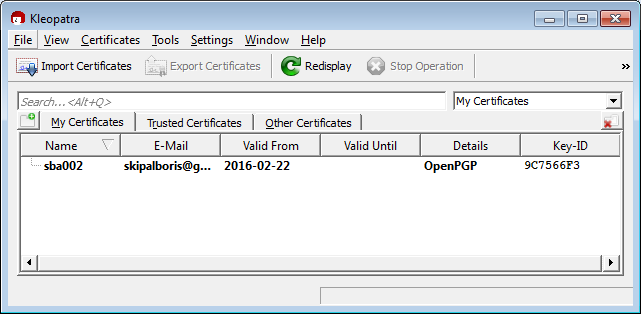
\includegraphics[width=1\linewidth]{res/step15}}
	\caption{Отображение новой ключевой пары.}
	\label{ris:step15}
\end{figure}


\subsection{Экспорт сертификата}
Для экспорта сертификата необходимо в графической оболочке \textit{"Kleopatra"} выполнить команду \textit{"File \begin{math}\to\end{math} Export Certificate"}. После чего откроется окно, в котором будет предложено выбрать название файла, где будет храниться сертификат (рисунок \ref{ris:step21})

\begin{figure}[h]
	\center{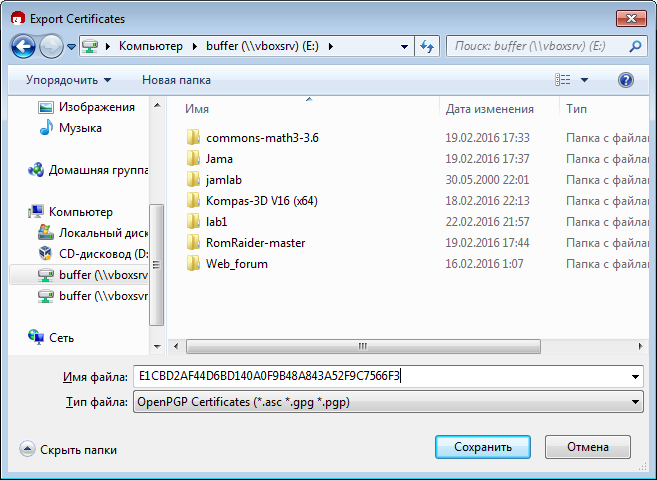
\includegraphics[width=1\linewidth]{res/step21}}
	\caption{Экспортирование сертификата.}
	\label{ris:step21}
\end{figure}

В данном случае файл будет называться\\"E1CBD2AF44D6BD140A0F9B48A843A52F9C7566F3.asc"

\subsection{Постановка ЭЦП на файл}
Перед тем, как поставить электронную цифровую подпись на файл, создадим текстовый файл "test.txt". Для того, что бы поставить свою ЭЦП на файл, необходимо выполнить команду \textit{"File \begin{math}\to\end{math} Sign/Encrypt Files"}. После чего появится окошко, в котором необходимо выбрать файл, для которого будет создаваться ЭЦП (рисунок \ref{ris:step31}).

\begin{figure}[h]
	\center{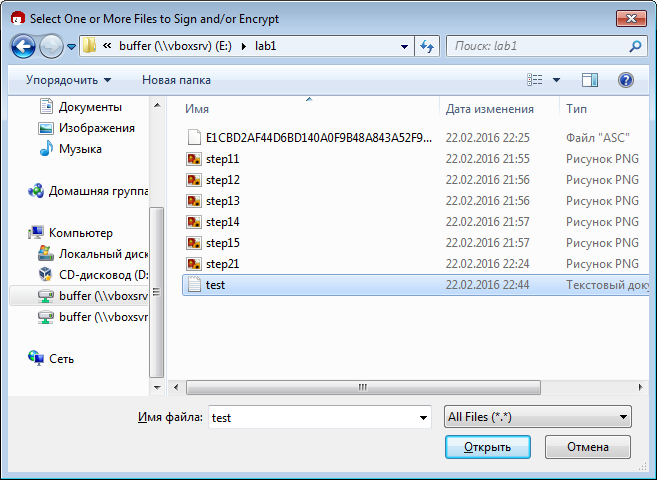
\includegraphics[width=1\linewidth]{res/step31}}
	\caption{Окно выбора файла.}
	\label{ris:step31}
\end{figure}

После чего помощника (рисунок \ref{ris:step32}), в котором необходимо выбрать пункт \textit{"Sign"} - создание цифровой подписи.

\begin{figure}[h]
	\center{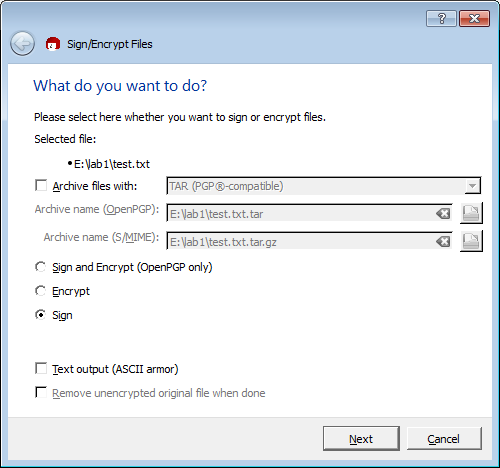
\includegraphics[width=1\linewidth]{res/step32}}
	\caption{Помощник создания ЭЦП.}
	\label{ris:step32}
\end{figure}

После чего появляется окошко, где необходимо подтвердить сертификат, которым будет подписываться файл (рисунок \ref{ris:step33}).

\begin{figure}[h]
	\center{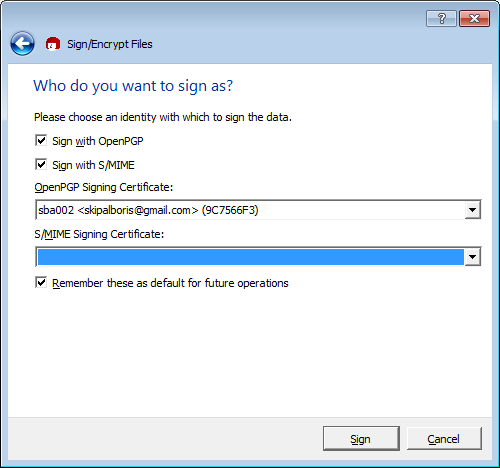
\includegraphics[width=1\linewidth]{res/step33}}
	\caption{Окно подтверждения сертификата.}
	\label{ris:step33}
\end{figure}

Затем необходимо аутентифицироваться при помощи пароля, заданного при создании ключа (рисунок \ref{ris:step34}).

\begin{figure}[h]
	\center{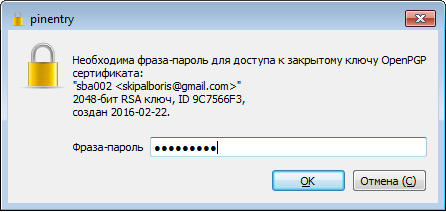
\includegraphics[width=0.7\linewidth]{res/step34}}
	\caption{Окно ввода пароля.}
	\label{ris:step34}
\end{figure}

После чего появится сообщение об успешном создании подписи (рисунок \ref{ris:step35}), а так же появится файл \textit{test.txt.sig}, в котором будет сохранена подпись.

\begin{figure}[h]
	\center{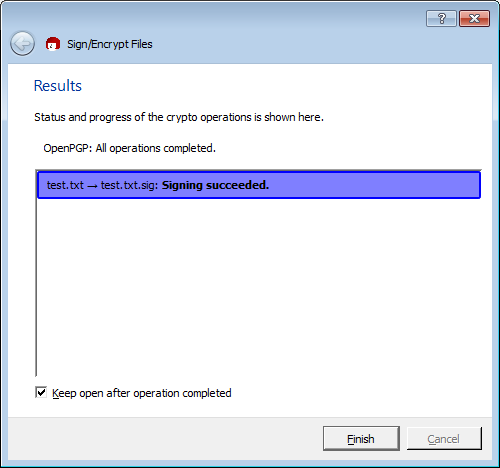
\includegraphics[width=1\linewidth]{res/step35}}
	\caption{Окно успешного создания подписи.}
	\label{ris:step35}
\end{figure}

Для проверки соответствия подписи выберем команду \textit{"File \begin{math}\to\end{math} Descript/ Verify Files"}. После чего необходимо выбрать сертификат, файл, который мы хотим проверить (в нашем случае test.txt), а так же файл с подписью (в нашем случае test.txt.sig). В случае успеха появится окошко, представленное на рисунке \ref{ris:step36}.

\begin{figure}[h]
	\center{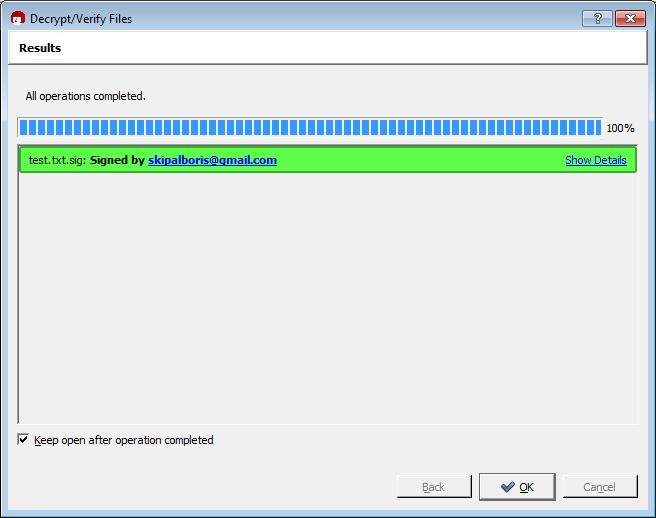
\includegraphics[width=1\linewidth]{res/step36}}
	\caption{Окно с результатами проверки подписи.}
	\label{ris:step36}
\end{figure}

\subsection{Импорт чужого сертификата}
Для импортирования чужого сертификата необходимо выполнить команду \textit{"File \begin{math}\to\end{math} Import Certificates"}. После чего откроется окно проводника, в котором необходимо выбрать чужой сертификат  (рисунок \ref{ris:step41}).

\begin{figure}[h]
	\center{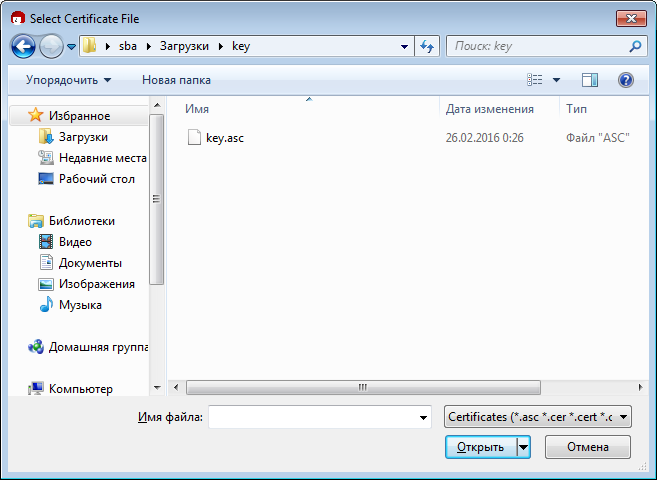
\includegraphics[width=1\linewidth]{res/step41}}
	\caption{Окно выбора файла сертификата.}
	\label{ris:step41}
\end{figure}

После этого новый сертификат можно увидеть во вкладке "Imported Certificates"  (рисунок \ref{ris:step42}).

\begin{figure}[h]
	\center{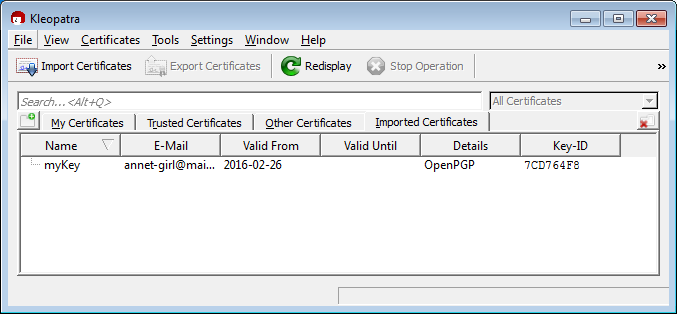
\includegraphics[width=1\linewidth]{res/step42}}
	\caption{Вкладка Imported Certificates.}
	\label{ris:step42}
\end{figure}

Для подписания чужого сертификата необходимо выполнить команду \textit{"File \begin{math}\to\end{math} Sign/ Encrypt Files"}. После чего появится окошко, в котором необходимо выбрать файл, для которого будет создаваться ЭЦП (в нашем случае необходимо указать сертификат другого человека). После чего для проверки необходимо выполнить пункт \textit{"File \begin{math}\to\end{math} Descript/ Verify Files"}. Результат представлен на рисунке \ref{ris:step43}.

\begin{figure}[h]
	\center{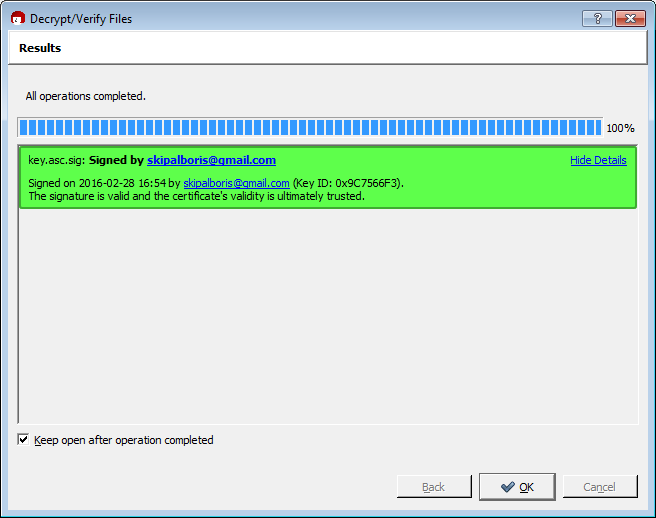
\includegraphics[width=1\linewidth]{res/step43}}
	\caption{Проверка подписи сертификата.}
	\label{ris:step43}
\end{figure}

Для того, что бы зашифровать файл открытым ключем, необходимо выбрать пункт \textit{"File \begin{math}\to\end{math} Sign/ Encrypt Files"}, после чего выбрать необходимый файл и выбрать пункт "Sign/ Encrypt" (рисунок \ref{ris:step44}).

\begin{figure}[h]
	\center{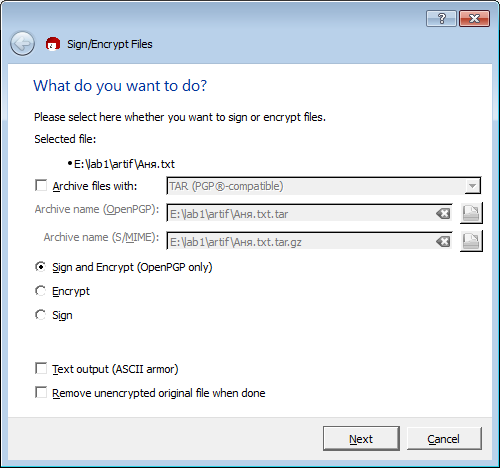
\includegraphics[width=1\linewidth]{res/step44}}
	\caption{Выбор параметров для шифрования файла.}
	\label{ris:step44}
\end{figure}

В следующем диалоговом окне нужно выбрать сертификат, при помощи которого будет подписываться и шифроваться файл (рисунок \ref{ris:step45}).

\begin{figure}[h]
	\center{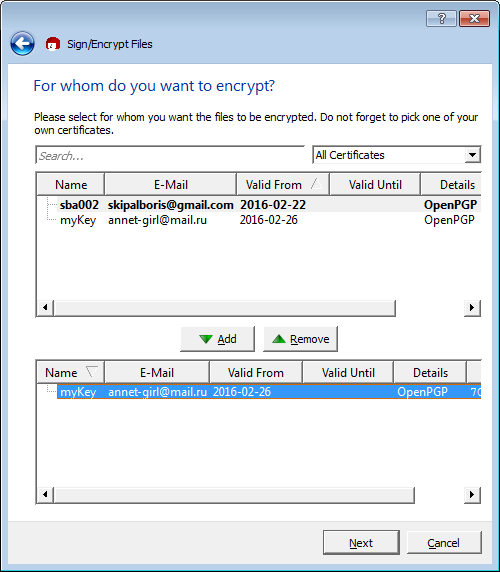
\includegraphics[width=1\linewidth]{res/step45}}
	\caption{Выбор сертификата для подписи и шифрования файла.}
	\label{ris:step45}
\end{figure}

После чего выбрать стандарт шифрования (в нашем случае OpenPGP) и нажать на кнопку "Sign/ Encrypt". После чего появится новый файл с расширением gpg (в нашем случае файл будет называться Аня.txt.gpg). Данный файл будет возможно расшифровать только при помощи закрытого сертификата другого человека. При попытке расшифровать файл тем сертификатом, при помощи которого он был зашифрован, получаем ошибку расшифровки (рисунок \ref{ris:step46}).

\begin{figure}[h]
	\center{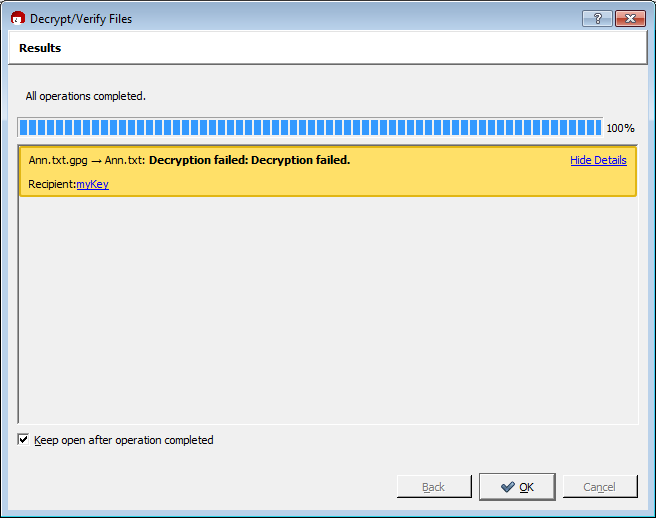
\includegraphics[width=1\linewidth]{res/step46}}
	\caption{Ошибка при попытке расшифровать файл открытым сертификатом другого человека.}
	\label{ris:step46}
\end{figure}

Попробуем расшифровать файл, зашифрованный другим человеком при помощи нашего сертификата. Для этого выберем свой сертификат, после чего выберем пункт \textit{"File \begin{math}\to\end{math} Descript/ Verify Files"} и нажмем на кнопку "Descript/ Verify". После чего нам предложат ввести пароль для того, что бы аутентифицироваться. В случае успеха увидим следующее сообщение (рисунок \ref{ris:step47}), которое сообщает о удачном завершении операции, а так же о том, кто зашифровал данный файл (в данном случае annet-girl@mail.ru). Так же появляется расшифрованный файл (в данном случае Боря.txt).

\begin{figure}[h]
	\center{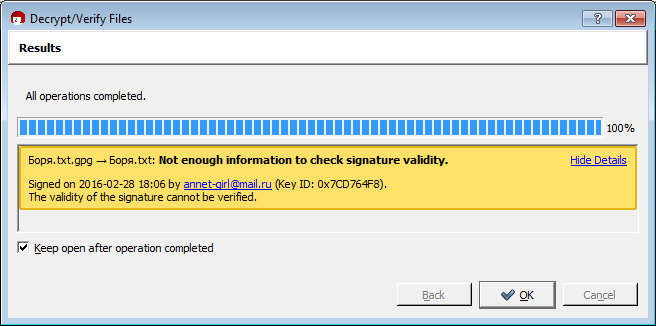
\includegraphics[width=1\linewidth]{res/step47}}
	\caption{Сообщение о удачной дешифровке файлов.}
	\label{ris:step47}
\end{figure}

\subsection{Использование консольных команд}
Вывод всех сертификатов происходит при помощи ключа "\--list-keys".
\begin{verbatim}
	C:\Users\sba>gpg --list-keys
	C:/Users/sba/AppData/Roaming/gnupg/pubring.gpg
	----------------------------------------------
	pub   2048R/9C7566F3 2016-02-22
	uid     [абсолютное] sba002 <skipalboris@gmail.com>
	sub   2048R/00808598 2016-02-22
	
	pub   2048R/7CD764F8 2016-02-25
	uid     [неизвестно] myKey <annet-girl@mail.ru>
	sub   2048R/4BECA6BD 2016-02-25
\end{verbatim}

Перед созданием сертификата необходимо создать ключевую пару при помощи ключа \--gen-key". В качестве типа ключа выберем RSA и RSA (по умолчанию), длину ключа выберем равной 2048 (значение по умолчанию), бесконечный срок действия. После этого нам будет предложено задать пароль для ключа и после этого ключевая пара будет создана.

\begin{verbatim}
C:\Users\sba\Downloads\lab1>gpg --gen-key
gpg (GnuPG) 2.0.29; Copyright (C) 2015 Free Software Foundation, Inc.
This is free software: you are free to change and redistribute it.
There is NO WARRANTY, to the extent permitted by law.

Выберите тип ключа:
(1) RSA и RSA (по умолчанию)
(2) DSA и Elgamal
(3) DSA (только для подписи)
(4) RSA (только для подписи)
Ваш выбор? 1
длина ключей RSA может быть от 1024 до 4096 бит.
Какой размер ключа Вам необходим? (2048) 2048
Запрошенный размер ключа - 2048 бит
Выберите срок действия ключа.
0 = без ограничения срока действия
<n>  = срок действия ключа - n дней
<n>w = срок действия ключа - n недель
<n>m = срок действия ключа - n месяцев
<n>y = срок действия ключа - n лет
Срок действия ключа? (0) 0
Срок действия ключа не ограничен
Все верно? (y/N) y

GnuPG необходимо составить ID пользователя в качестве идентификатора ключа.

Ваше настоящее имя: SkripalBoris
Адрес электронной почты: skipalboris@yandex.ru
Комментарий: none
Вы выбрали следующий ID пользователя:
"SkripalBoris (none) <skipalboris@yandex.ru>"

Сменить (N)Имя, (C)Комментарий, (E)Адрес или (O)Принять/(Q)Выход? O
Для защиты закрытого ключа необходима фраза-пароль.

Необходимо получить много случайных чисел. Желательно, чтобы Вы
в процессе генерации выполняли какие-то другие действия (печать
на клавиатуре, движения мыши, обращения к дискам); это даст генератору
случайных чисел больше возможностей получить достаточное количество энтропии.
Необходимо получить много случайных чисел. Желательно, чтобы Вы
в процессе генерации выполняли какие-то другие действия (печать
на клавиатуре, движения мыши, обращения к дискам); это даст генератору
случайных чисел больше возможностей получить достаточное количество энтропии.
gpg: ключ 3729EB59 помечен как абсолютно доверенный.
открытый и закрытый ключи созданы и подписаны.

gpg: проверка таблицы доверия
gpg: требуется 3 с ограниченным доверием, 1 с полным, модель доверия PGP
gpg: глубина: 0  верных:   2  подписанных:   0  доверие: 0-, 0q, 0n, 0m, 0f, 2u
pub   2048R/3729EB59 2016-02-29
Отпечаток ключа = D675 32A4 0148 164D 1BBC  C95C 6460 E810 3729 EB59
uid     [абсолютное] SkripalBoris (none) <skipalboris@yandex.ru>
sub   2048R/100C8383 2016-02-29

C:\Users\sba\Downloads\lab1>gpg --list-keys
C:/Users/sba/AppData/Roaming/gnupg/pubring.gpg
----------------------------------------------
pub   2048R/9C7566F3 2016-02-22
uid     [абсолютное] sba002 <skipalboris@gmail.com>
sub   2048R/00808598 2016-02-22

pub   2048R/7CD764F8 2016-02-25
uid     [неизвестно] myKey <annet-girl@mail.ru>
sub   2048R/4BECA6BD 2016-02-25

pub   2048R/3729EB59 2016-02-29
uid     [абсолютное] SkripalBoris (none) <skipalboris@yandex.ru>
sub   2048R/100C8383 2016-02-29
\end{verbatim}

Для создания сертификата необходимо использовать два ключа: "\--output" для задания выходного файла, и "\--gen-revoke" для задания ключевой пары.

\begin{verbatim}
C:\Users\sba\Downloads\lab1>gpg --output Skripal.asc --gen-revoke SkripalBoris

sec  2048R/3729EB59 2016-02-29 SkripalBoris (none) <skipalboris@yandex.ru>

Создать сертификат отзыва данного ключа? (y/N) y
Укажите причину отзыва:
0 = Причина не указана
1 = Ключ был раскрыт
2 = Ключ заменен другим
3 = Ключ больше не используется
Q = Отмена
(Скорее всего, Вы здесь выберете 1)
Ваше решение? 0
Введите необязательное пояснение; закончите пустой строкой:
>
Причина отзыва: Причина не указана
(Пояснения отсутствуют)
Все правильно? (y/N) y

Необходима фраза-пароль для доступа к закрытому ключу пользователя: "SkripalBori
s (none) <skipalboris@yandex.ru>"
2048-битный ключ RSA, ID 3729EB59, создан 2016-02-29

Сертификат отзыва создан.
\end{verbatim}

Для симметричного шифрования файла используется ключ "\--symmetric". Создадим файл "SkripalSec.txt" и зашифруем его при помощи закрытого ключа.

\begin{verbatim}
	gpg --symmetric SkripalSec.txt
\end{verbatim}

После этого в папке появится файл SkripalSec.txt.gpg

\begin{verbatim}
dir

28.02.2016  17:20    <DIR>          .
28.02.2016  17:20    <DIR>          ..
28.02.2016  16:52                 7 SkripalSec.txt
28.02.2016  17:20                60 SkripalSec.txt.gpg
\end{verbatim}

Для расшифровки файла необходимо использовать ключ "\--decrypt".

\begin{verbatim}
C:\Users\sba\Downloads\lab1>gpg --decrypt SkripalSec.txt.gpg
gpg: данные зашифрованы алгоритмом CAST5
gpg: зашифровано одной фразой-паролем
Hello!
gpg: ВНИМАНИЕ: целостность сообщения не защищена
\end{verbatim}
	
\end{document}